\documentclass[11pt,addpoints,answers]{exam}

\usepackage[top=0.5in, left=0.75in, right=0.75in, bottom=.75in]{geometry}
\usepackage{amsmath,amsfonts,nicefrac, amssymb,amsxtra}
\usepackage{mathtools}
\usepackage{multicol}
\usepackage{pdfpages}
\usepackage{setspace}
\usepackage{enumitem}

%\usepackage{mathexam}
%\usepackage{latexsym}
%\usepackage[square, comma, sort&compress, numbers]{natbib}
%\usepackage{moresize}
%\usepackage{algpseudocode}
\usepackage{stmaryrd}
%\usepackage{enumitem}
%\renewcommand{\theenumi}{\alph{enumi}}
\usepackage{tabularx,ragged2e,booktabs,caption}
\usepackage{epstopdf}
\usepackage{epsfig}
\usepackage{setspace}
\usepackage{tikz,pgfplots}
\usetikzlibrary{arrows.meta}
\usetikzlibrary{arrows,decorations.markings}
\pgfplotsset{compat=1.14}
\usepgfplotslibrary{units}
\pgfplotsset{soldot/.style={color=black,only marks,mark=*}}
\pgfplotsset{holdot/.style={color=black,fill=white,only marks,mark=*}}
\usepackage{polynom}
\usepackage{enumerate}
\usepackage{graphicx,wrapfig,lipsum}
\allowdisplaybreaks


\usepackage[utf8]{inputenc}
\usetikzlibrary{decorations}
\usetikzlibrary{decorations.pathreplacing}
%\usepackage{fancyhdr}
\usepackage{array}
\usepackage{parskip}

\renewcommand{\arraystretch}{1.2}
\renewcommand\partlabel{(\thequestion.\arabic{partno})}

\newcommand{\emptybox}[2][\textwidth]{%
  \begingroup
  \setlength{\fboxsep}{-\fboxrule}%
  \noindent\framebox[#1]{\rule{0pt}{#2}}%
  \endgroup
}

\pgfplotsset{compat=1.14}


\begin{document}
\noindent {\Large Quiz, Fall Week 3 \hfill Name: \underline{\hspace{7cm}}}

\noindent {\normalsize {Points possible: \numpoints      \hfill Math 1050-90, Fall 2021, Due 9/14 at 11:59 p.m.}}

{\small \noindent \textbf{Rules/Suggestions:} Write with a dark pencil, so that your work is visible.  \textbf{You are graded on your work, not just answers. Even if you do calculations in your head or on scratch, show work if space is provided. } Write the final answer in the box.

Notes: You are on your honor for this to be your own work.  (You can ask for help on quiz material, but you should not ask for help on specific problems.) }
\begin{questions}
\setlength\columnsep{1cm}
\question Find the degree, leading term, leading coefficient, constant term, and end behavior of the given polynomial.
\[f(x) = 12 + 7x^2 - 5x^3-2x^6\]
\begin{parts}
\part[5] Rewrite the polynomial in order of descending degree.  What is the  degree, leading term, leading coefficient, and constant term of $f$?

\begin{flushleft}\fbox{%
\begin{minipage}{6.25 in}
\hspace{1in}\\[1.5ex]
Answers: \quad \quad $f(x) =$
\begin{multicols}{2}
    \begin{itemize}
        \item degree: \underline{\hspace{3cm}}
        \vspace*{0.25in}
        \item leading term: \underline{\hspace{2cm}}
        \columnbreak
        \item leading coefficient:\underline{\hspace{1.5cm}}
        \vspace*{0.25in}
        \item constant term:\underline{\hspace{2.5cm}} \\ [1ex]
    \end{itemize}
\end{multicols}
\end{minipage}}\end{flushleft}

\part[10] Explain how to figure out the end behavior of $f$, then state the end behavior.\\

\begin{multicols}{2}
\begin{flushleft}\fbox{%
\begin{minipage}{2.75in}
    \hspace{1in}\\[1.5ex]
    Explanation:
    \vspace*{1in}
    \begin{itemize}
        \item As $x\longrightarrow-\infty$, $f(x)\longrightarrow$ \underline{\hspace{1.75cm}}\\ [1.5ex]
    \end{itemize}
\end{minipage}}\end{flushleft}

\begin{flushleft}\fbox{%
\begin{minipage}{2.75in}
    \hspace{1in}\\[1.5ex]
    Explanation:
    \vspace*{1in}
    \begin{itemize}
        \item As $x\longrightarrow\infty$, $f(x)\longrightarrow$ \underline{\hspace{1.75cm}}\\ [1.5ex]
    \end{itemize}
\end{minipage}}\end{flushleft}
\end{multicols}
\end{parts}
\vspace{0.2in}

\question For $g(x)= 2x(x+4)^2(x+1)(x-5)$, fill in the following information.
\begin{multicols}{2}
\begin{parts}
\part[6] All the zeros/roots:  \\
\vspace*{2cm}
\part[2]  As $x\rightarrow-\infty$, $g(x)\rightarrow$ \underline{\hspace{1cm}} \\
\columnbreak
\part[4] $y$-intercept: \\ (Write an ordered pair) \\
\vspace*{2cm}
\part[2]   As $x\rightarrow \infty$, $g(x)\rightarrow$ \underline{\hspace{1.4cm}}\\
\columnbreak
\part[10] Sketch its graph. Label with numbers the values of zeros/$x$-intercepts.\\
\vspace{.2cm}
\scalebox{.7}{\begin{tikzpicture}[>=latex]
\begin{axis}[
	ticks=none,
	axis x line=center,
	axis y line=center,
	xtick={-7,-5,...,6,7},
	ytick={-8,-7,...,8},
	xmin=-7,
	xmax=7,
	ymin=-8,
	ymax=8,
	xticklabel style={xshift=-0.5ex},
	yticklabel style={yshift=-0.5ex},
	xlabel={$x$},
	ylabel={$y$},
	xlabel style={right},
	ylabel style={above},
	%grid=both,
	scale=1.4, transform shape]
\end{axis}
\end{tikzpicture}}
\vspace{.2cm}
\columnbreak
\part[2] Using your graph, where is $g(x)> 0$?  Write your answer with interval notation. \\
\vspace{.2cm}

\underline{\hspace{7cm}}\\
\end{parts}\end{multicols}

\question[12] Write $f(x) = x^4+4x^3-7x^2-34x-24$ in factored form.  Use the fact that both $(x+1)$ and $(x+2)$ are factors of $f$.

\vspace*{1.5in}
\begin{flushright}\fbox{%
\begin{minipage}{4 in}
\hspace{1in}\\[1ex]
Answer:\\[1ex]
\indent{\quad} $f(x)=$\\
\end{minipage}}\end{flushright}

\question[12]  Find all the zeros of $f(x) = x^4-3x^3+x^2-27x+28$.  A graph of $f$ is provided as a hint.  Simplifying the roots and fractions in answers is optional.

\scalebox{.9}{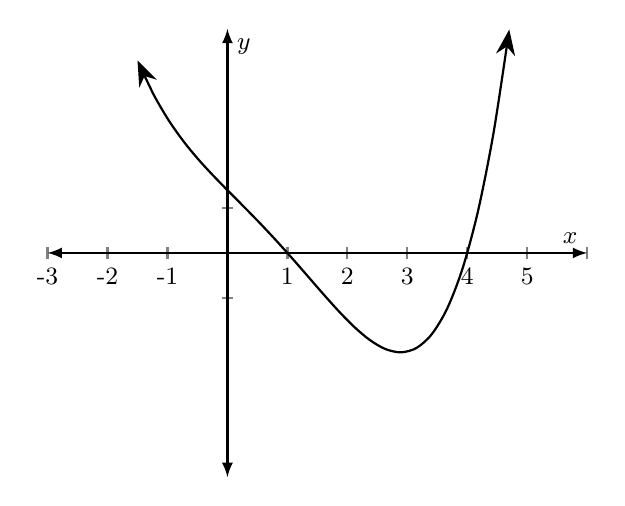
\begin{tikzpicture}
\begin{axis}[
every tick label/.append style={font=\small},
  axis lines=middle,
  grid=major,  major grid style={line width=.2pt,draw=white!50},   axis line style={latex-latex,line width=.8pt,black!100},
  xmin=-3,
  xmax=6,
  ymin=-100,
  ymax=100,
  xlabel=\small{$x$},
 ylabel=\small{$y$},
  xtick={-3,-2,-1,1,2,3,4,5,6},
  ytick={-20,0,20},
  yticklabels=\empty,
  xticklabels={-3,-2,-1,1,2,3,4,5},
  tick style={thick}]
\addplot[<->,{Stealth[scale=1.4]}-{Stealth[scale=1.4]}, smooth, domain=-1.5:4.7, thick] {x^4-3*x^3+x^2-27*x+28};
\end{axis}
\end{tikzpicture}}

\begin{flushright}\fbox{%
\begin{minipage}{4 in}
\hspace{1in}\\[1ex]
Answer:\\[3ex]
\end{minipage}}\end{flushright}
\vspace{.2in}

\question Given $f(x) = x^4+x^3-18x^2-52x-40$.

\begin{parts}
\part[5] Write the possible rational roots according to the \textbf{Rational Zero Theorem}.

\begin{flushleft}\fbox{%
\begin{minipage}{6.3in}
\hspace{0.5in}\\[.2ex]
Answer:\\[1ex]
\end{minipage}}\end{flushleft}

\part[8] Use synthetic division to test possible rational roots.  Test the possible values until you find a root.  When you find one, circle the work.   If you are lucky and find it the first time, show one more test of a different value.
\vspace{1.5in}
\part[10] Find ALL the zeros of $f(x) = x^4 + x^3 - 18x^2 - 52x - 40$.  Write the function in fully factored form.
\vspace*{1.5in}
\begin{flushright}\fbox{%
\begin{minipage}{3 in}
\hspace{1in}\\[.8ex]
Answer:\\[1.8ex]
\end{minipage}}\end{flushright}
\end{parts}

\question[12] Find the real solutions of the polynomial equation $x^3+14=6x^2+9x$.  Write your answers as a list.
\vspace*{1.5in}
\begin{flushright}\fbox{%
\begin{minipage}{3 in}
\hspace{1in}\\[.8ex]
Answer:\\[1.8ex]
\end{minipage}}\end{flushright}

\end{questions}

\end{document}
